% This is "sig-alternate.tex" V2.1 April 2013
% This file should be compiled with V2.5 of "sig-alternate.cls" May 2012
%
% This example file demonstrates the use of the 'sig-alternate.cls'
% V2.5 LaTeX2e document class file. It is for those submitting
% articles to ACM Conference Proceedings WHO DO NOT WISH TO
% STRICTLY ADHERE TO THE SIGS (PUBS-BOARD-ENDORSED) STYLE.
% The 'sig-alternate.cls' file will produce a similar-looking,
% albeit, 'tighter' paper resulting in, invariably, fewer pages.
%
% ----------------------------------------------------------------------------------------------------------------
% This .tex file (and associated .cls V2.5) produces:
%       1) The Permission Statement
%       2) The Conference (location) Info information
%       3) The Copyright Line with ACM data
%       4) NO page numbers
%
% as against the acm_proc_article-sp.cls file which
% DOES NOT produce 1) thru' 3) above.
%
% Using 'sig-alternate.cls' you have control, however, from within
% the source .tex file, over both the CopyrightYear
% (defaulted to 200X) and the ACM Copyright Data
% (defaulted to X-XXXXX-XX-X/XX/XX).
% e.g.
% \CopyrightYear{2007} will cause 2007 to appear in the copyright line.
% \crdata{0-12345-67-8/90/12} will cause 0-12345-67-8/90/12 to appear in the copyright line.
%
% ---------------------------------------------------------------------------------------------------------------
% This .tex source is an example which *does* use
% the .bib file (from which the .bbl file % is produced).
% REMEMBER HOWEVER: After having produced the .bbl file,
% and prior to final submission, you *NEED* to 'insert'
% your .bbl file into your source .tex file so as to provide
% ONE 'self-contained' source file.
%
% ================= IF YOU HAVE QUESTIONS =======================
% Questions regarding the SIGS styles, SIGS policies and
% procedures, Conferences etc. should be sent to
% Adrienne Griscti (griscti@acm.org)
%
% Technical questions _only_ to
% Gerald Murray (murray@hq.acm.org)
% ===============================================================
%
% For tracking purposes - this is V2.0 - May 2012

\documentclass{sig-alternate-05-2015}

\usepackage{amsmath}
\usepackage{algorithmic}
\usepackage{subfigure}
\usepackage{graphicx}
\usepackage{multirow}
\usepackage{algorithm}
\usepackage{color}
\usepackage{amsmath}
\usepackage{mathabx}

\newcommand{\squishlist}{
    \begin{list}{$\bullet$}
    { \setlength{\itemsep}{0pt}
        \setlength{\parsep}{3pt}
        \setlength{\topsep}{3pt}
        \setlength{\partopsep}{0pt}
        \setlength{\leftmargin}{1.5em}
        \setlength{\labelwidth}{1em}
        \setlength{\labelsep}{0.5em} } }

\newcommand{\squishlisttwo}{
    \begin{list}{$\bullet$}
        { \setlength{\itemsep}{0pt}
            \setlength{\parsep}{0pt}
            \setlength{\topsep}{0pt}
            \setlength{\partopsep}{0pt}
            \setlength{\leftmargin}{2em}
            \setlength{\labelwidth}{1.5em}
            \setlength{\labelsep}{0.5em} } }

\newcommand{\squishend}{
    \end{list}  }

\begin{document}

% Copyright
\setcopyright{acmcopyright}
%\setcopyright{acmlicensed}
%\setcopyright{rightsretained}
%\setcopyright{usgov}
%\setcopyright{usgovmixed}
%\setcopyright{cagov}
%\setcopyright{cagovmixed}


% DOI
%\doi{10.475/123_4}

% ISBN
%\isbn{123-4567-24-567/08/06}

%Conference
%\conferenceinfo{PLDI '13}{June 16--19, 2013, Seattle, WA, USA}

%\acmPrice{\$15.00}

%
% --- Author Metadata here ---
%\conferenceinfo{WOODSTOCK}{'97 El Paso, Texas USA}
%\CopyrightYear{2007} % Allows default copyright year (20XX) to be over-ridden - IF NEED BE.
%\crdata{0-12345-67-8/90/01}  % Allows default copyright data (0-89791-88-6/97/05) to be over-ridden - IF NEED BE.
% --- End of Author Metadata ---
\title{Setting a perfect goal to succeed in Kickstarter:\\ 
A non-linear regression model}
%
% You need the command \numberofauthors to handle the 'placement
% and alignment' of the authors beneath the title.
%
% For aesthetic reasons, we recommend 'three authors at a time'
% i.e. three 'name/affiliation blocks' be placed beneath the title.
%
% NOTE: You are NOT restricted in how many 'rows' of
% "name/affiliations" may appear. We just ask that you restrict
% the number of 'columns' to three.
%
% Because of the available 'opening page real-estate'
% we ask you to refrain from putting more than six authors
% (two rows with three columns) beneath the article title.
% More than six makes the first-page appear very cluttered indeed.
%
% Use the \alignauthor commands to handle the names
% and affiliations for an 'aesthetic maximum' of six authors.
% Add names, affiliations, addresses for
% the seventh etc. author(s) as the argument for the
% \additionalauthors command.
% These 'additional authors' will be output/set for you
% without further effort on your part as the last section in
% the body of your article BEFORE References or any Appendices.

\numberofauthors{2} %  in this sample file, there are a *total*
% of EIGHT authors. SIX appear on the 'first-page' (for formatting
% reasons) and the remaining two appear in the \additionalauthors section.
%
\author{
% You can go ahead and credit any number of authors here,
% e.g. one 'row of three' or two rows (consisting of one row of three
% and a second row of one, two or three).
%
% The command \alignauthor (no curly braces needed) should
% precede each author name, affiliation/snail-mail address and
% e-mail address. Additionally, tag each line of
% affiliation/address with \affaddr, and tag the
% e-mail address with \email.
%
% 1st. author
\alignauthor
Thanh Tran\\
       \affaddr{Department of Computer Science}\\
       \affaddr{Utah State University}\\
       \affaddr{Logan, UT 84341}\\
       \email{thanh.tran@aggiemail.usu.edu}
% 2nd. author
\alignauthor
Hongkyu Choi\\
       \affaddr{Utah State University}\\
       \affaddr{Utah State University}\\
       \affaddr{Logan, UT 84341}\\
       \email{hongkyu.choi@aggiemail.usu.edu}
}

% There's nothing stopping you putting the seventh, eighth, etc.
% author on the opening page (as the 'third row') but we ask,
% for aesthetic reasons that you place these 'additional authors'
% in the \additional authors block, viz.

% Just remember to make sure that the TOTAL number of authors
% is the number that will appear on the first page PLUS the
% number that will appear in the \additionalauthors section.

\maketitle

\begin{abstract}
	To find the answer of how to succeed in crowdfunding, we find many previous works which are mainly focused on to recommend appropriate investors to a project or investigate more influential features on its success. However, in this paper, we would like to suggest a way to set a perfect goal with introducing a regression model. Establishing a goal appropriate is essential for project to success eventually as well as predicting the number of backers a certain Kickstarter project.
	
	Our proposed model show better performance than existing algorithm(Simple linear regression and XgBoost). It returns RMSE(Root Mean Square Error) 23.7 and 1,659, prediction for the number of backer and funding respectively.
\end{abstract}
\section{Introduction}
Why is this an interesting question to ask and why would we care about the answer to this question or a solution to set a perfect goal? The Kickstarter policy is one or nothing. It means that if the amount of final pledged money is equal or higher than the goal, the fundraising campaign is successful. Otherwise, the fundraising campaign is fail and the creator receives nothing. If the creator overestimate the project goal, they will be fail, but if the creator set the project goal too low, they may not get attraction from community and gain less amount of money. Hence, predicting the amount of money or the number of backers are very important for Kickstarter creators to raise fund.

To our knowledge, There is only one research work try to predict how much fund a Kickstarter project can receive. Particularly, researchers at \cite{chung2015long} convert the problem of predicting the amount of final pledged money into classification problem by dividing such amount of final pledged money into different range. So the problem of predicting how much fund a Kickstarter project can receive will be the problem of predicting which range of money the project can receive.

Comparing to this work, our work is totally different, instead of predicting the range of final pledged fund, we build regression model to predict exactly the amount of money as well as the number of backers given a certain Kickstarter project.

Our contributions (or research questions) in this proposal are:
\begin{itemize}
\item Understand the influence of multiple factors toward the number of backers and the amount of final pledged money that a certain project can receive. We will show statistic values to illustrate for such influence.
\item Given a project, we build a model to predict how much pledged fund the creator can receive
\item Building a model to predict how many backers will fund for the project.
\end{itemize}
\section{Related Works}
\section{Dataset}
\section{Analysis}

\section{Features}
In this section, we propose some features which are useful to develop two predictors of how much funding and the number of backers. We groups all our proposed features in different traits:
\subsection{Project-based features}
Given a Kickstarter project's page, we extracted all following features:
\begin{itemize}
	\item number of project's comments,
	\item number of updates
	\item number of rewards,
	\item number of images,
	\item number of videos,
	\item number of faqs,
	\item the goal of the project
	\item category of the project
	\item duration of fund raising of the project
	\item smog score of all rewards: we extracted all rewards' description of the Kickstarter project then grouped them into one document. Next, we computed the smog score of the document and considered it as smog score of all rewards' description.
	\item number of reward sentences,
	\item number of main sentences,
	\item smog score of project's description: we extracted the project's description and computed its smog score.
	\item smog score of biography description
\end{itemize}
SMOG score of a document show how well the document is written. The higher the SMOG score, the better the document was written. The formula to compute SMOG score is as following:
\[
	grade = 1.0430\sqrt{\#polysyllables * \frac{30}{\#sentences}} + 3.1291	
\]
\subsection{Creator-based features}
We proposed some features related to Kickstarter creators as following:
\begin{itemize}
	\item successful rate of all previous backed projects: given a Kickstarter project, we collected all projects that the creator backed and calculate the average successful rates of these backed projects. Our intuition behind it is that if the creator backed many successful projects, he may have an idea of how to get more fund and attract more backers.
	\item previous successful rate of creator's project: we first collected all projects that the creator launched. Then we calculate average successful rate of such projects. The intuition is that if the creator successfully raised fund in many projects, he may have many experience in raising more fund or getting interest from backers.
	\item number of created projects: as mentioned in \cite{chung2015long}, the more projects that creator launched, the more successful he is in raising fund.
\end{itemize}
\subsection{Social network - based features}
Social promotion is an effective way to promote Kickstarter project and attract more funding. Hence, we use some features related to social communication of the creator as following:
\begin{itemize}
	\item number of Facebook friends
	\item connected to Twitter? (binary feature)
	\item connected to Facebook? (binary feature)
	\item connected to Youtube? (binary feature)
	\item how many websites that the creator has?
\end{itemize}
\subsection{Feature Selection}
In this section, we present our approach to remove non-significant features. We first remove all highly correlated features by setting cutoff value of 0.7. That is, if a feature has correlation score of greater than or equal to 0.7 with another one, we remove such feature. After removing all the highly correlated features, we obtained the correlation matrix as shown in Figure \ref{fig:CorrelationMatrix}. 

Among all the rest of uncorrelated features, we would like to keep only significant features. In order to do so, we sequentially choose p features (p = 1,..,n) and calculate the stepAIC value as following:
\[
	stepAIC = nln(SSE_p) - nln(n) + 2p
\]
where \emph{n} is the total number of features, $SSE_p$ is the sum of square error (SSE) that we got by building the model with \emph{p} features. We will choose the subset of all n features which minimize stepAIC score.

\begin{figure}%[!ht]
	\centering
	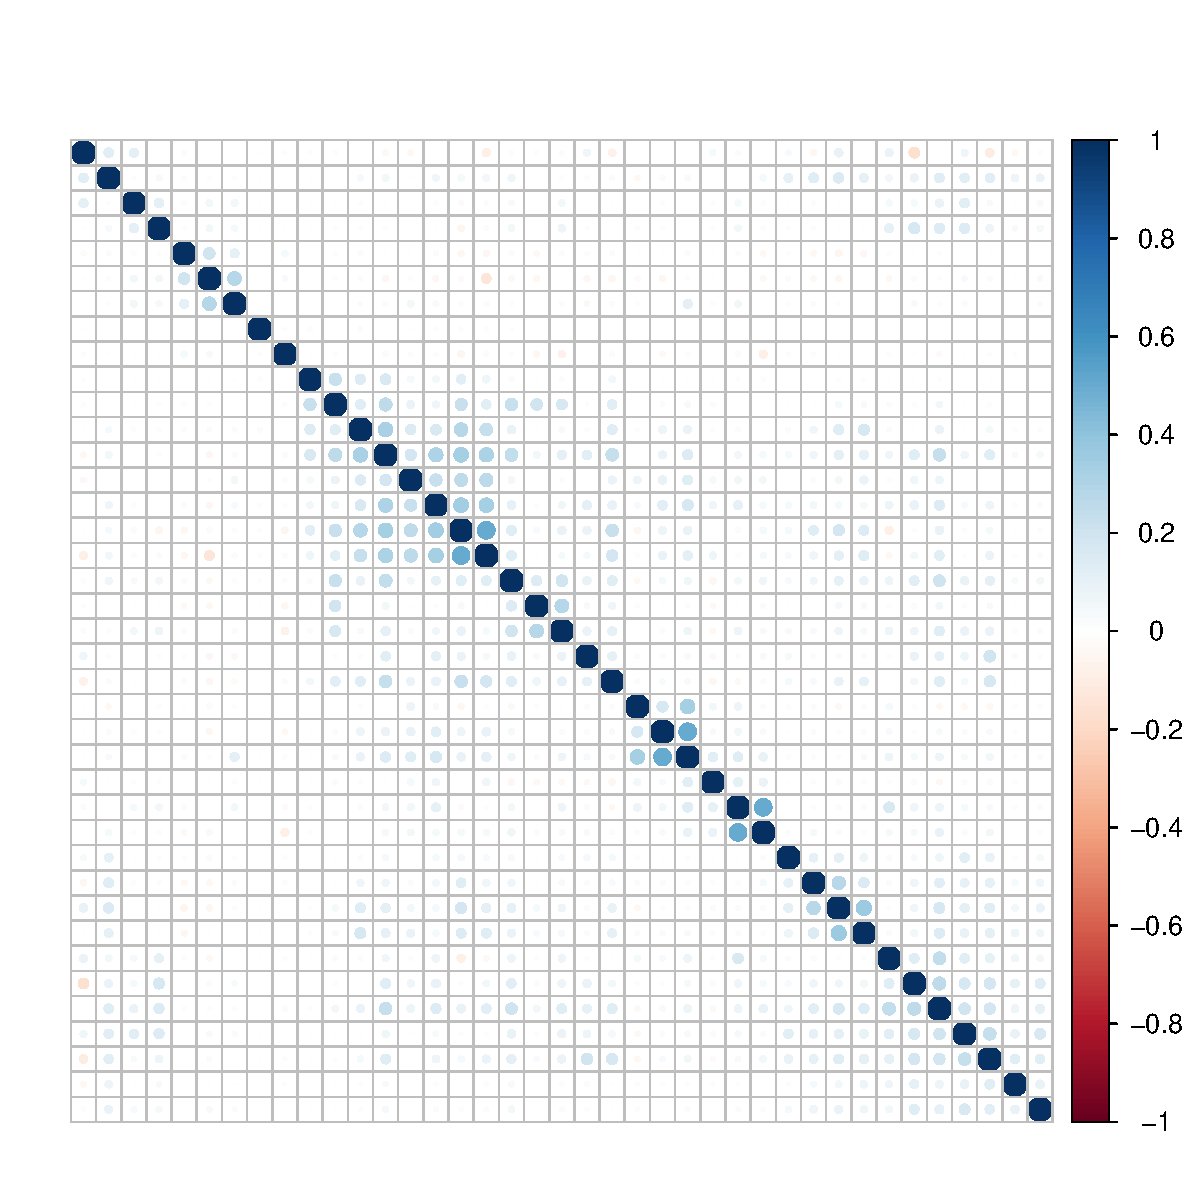
\includegraphics[width=\linewidth]{figs/CorrelationMatrix.pdf}
	\caption{Correlation matrix of all features after removing highly correlated features}
	\label{fig:CorrelationMatrix}
	\vspace{-10pt}
\end{figure}

\section{Our proposed non-linear Regression model}
Fitting a linear model for our problems of predicting the number of backers and the amount of funding for a given Kickstarter project may not be always helpful since the correlation between all features and response could not be linearity.  Hence, we proposed a non-linear model as following:
\begin{equation}
\begin{aligned}
Y^\lambda = \beta_0 + \beta^TX + \epsilon
\end{aligned}
\end{equation}
Here, $\epsilon$ is the random error and follows normal distribution $N(0, \sigma^2)$. The power of this model is that with different value of $\lambda$, we have different curvature function. For instance, when $\lambda=0.5$, we have the function:
\begin{equation}
\label{equa:LambdaOf2}
\begin{aligned}
\widehat{Y}^{1/2} = \beta_0 + \beta^TX = X\beta
\end{aligned}
\end{equation}

The Equation (\ref{equa:LambdaOf2}) can be rewritten as following:
\begin{equation}
\label{equa:LambdaOf2Convert}
\begin{aligned}
\widehat{Y} = (\beta_0 + \beta^TX) ^2 = (X\beta)^2
\end{aligned}
\end{equation}

Now, the Equation (\ref{equa:LambdaOf2Convert}) is a quadratic function, not a linear model. Similarly, when $\lambda=1/3$, we have a cubic function that get through all points.

The next problem is how we can find out the best value of $\lambda$ for the model? In order to seek the answer for that question, we first find out the likelihood function of our proposed model. Given features' value and the real value \emph{Y}, our proposed model generated predicted value $\widehat{Y}$.  Our goal is to minimize the optimized function of error:
\[
	\min error^2 = \sum_{i=1}^{n}{(Y_i^\lambda -\widehat{Y_i})^2}
\]

We assume that the error follows normal distribution N(0, $\sigma^2$). The probability density of $error_i$ of \emph{ith} observation is given as following:
\begin{equation}
\label{equa:densityProbability}
\begin{aligned}
	f(error|\mu, \sigma^2) 	&= \frac{1}{\sigma\sqrt{2\pi}}e^{-\frac{error_i^2}{\sigma^2}} \\
						&= \frac{1}{\sigma\sqrt{2\pi}}e^{-\frac{{(Y_i^\lambda -\widehat{Y_i})^2}}{\sigma^2}} \\
						&= \frac{1}{\sigma\sqrt{2\pi}}e^{-\frac{{(Y_i^\lambda -X\beta)^2}}{\sigma^2}}
\end{aligned}			
\end{equation}

Given Equation (\ref{equa:densityProbability}), the loglikelihood function of error is:
\begin{equation}
\label{equa:LogLikelihoodFunction}
\begin{aligned}
log(L) = -\frac{n}{2}kig(2\pi) -nlog(\sigma) - \frac{1}{2\sigma^2}\sum_{i=1}^{n}{[Y_i^\lambda - X\beta]^2}  \\ + (\lambda-1) \sum_{i=1}^{n}log(Y_i)
\end{aligned}
\end{equation}

Here, $\sigma$ can be estimated by MSE obtained in the regression model. And the problem of finding the best value of $\lambda$ will become the problem of maximizing loglikelihood function given in Equation (\ref{equa:LogLikelihoodFunction}). 




\section{Experiments and Result}

In this section, we described all our experimental settings which are used in following sections for predicting how many backers will back for a certain Kickstarter project and how much funding that the project can receive.

\subsection{Experiment Setting}

\textbf{Dataset:} With all 151,608 projects, we see projects with extremely high amount of funding or number of backers as outliers and remove them. We also consider projects with the goal less than \$100 as noisy projects and should remove them. As a result, from 151,608 projects as origin, we filtered out 36,731 outliers and the rest contains only 114,877 projects.

\textbf{Measure:} In all below experiments, we evaluate the result based on root mean square error (\emph{RMSE}). \emph{RMSE} is a common measure to evaluate the average difference between the predicted values and  real values. The formula to compute RMSE is given as following:
\[
	RMSE = \sqrt{\frac{\sum_{i=1}^{n}{(Y_i-\widehat{Y_i})^2}}{n}}
\]
where $Y_i$ is the real value of response at observation \emph{i} and $\widehat{Y_i}$ is the estimated value of response at observation \emph{i}.

\textbf{Features Normalization:} Since different features have different scale, the features with larger scale may have lower coefficient then ones with smaller scale and may cause larger error. In order to avoid the problem, we normalized all features into [0,1] scale by applying softmax normalization. The formula of softmax normalization is given as following:
\[
	x_{ij}\prime = \frac{1}{1 + e^{-\frac{x_{ij}-\mu_i}{\sigma_i}}}
\]
where $x_ij$ is the value of \emph{ith} feature at observation \emph{j}, $\mu_i$ and $\sigma_i$ are the mean and the standard deviation of all the values of \emph{ith} feature, respectively.

\textbf{Predicting how many backers will back for a Kickstarter project and how much funding the project can receive:} In this experiment, we used our proposed features and build the models to predict how many backers will back for a Kickstarter project and how much funding the project can receive based on 3 approaches: linear regression, extreme gradient boosting for linear regression and our regression model. 
\subsection{Experiment Result}
For our proposed regression model, we first find out the best value of $\lambda$ by maximize the loglikelihood function given above section

\begin{figure*}%[!ht]
	\centering
	\subfigure[Value of $\lambda$ in regression model for predicting number of backers] % caption for subfigure a
	{
		\label{fig:lambdaBackers}
		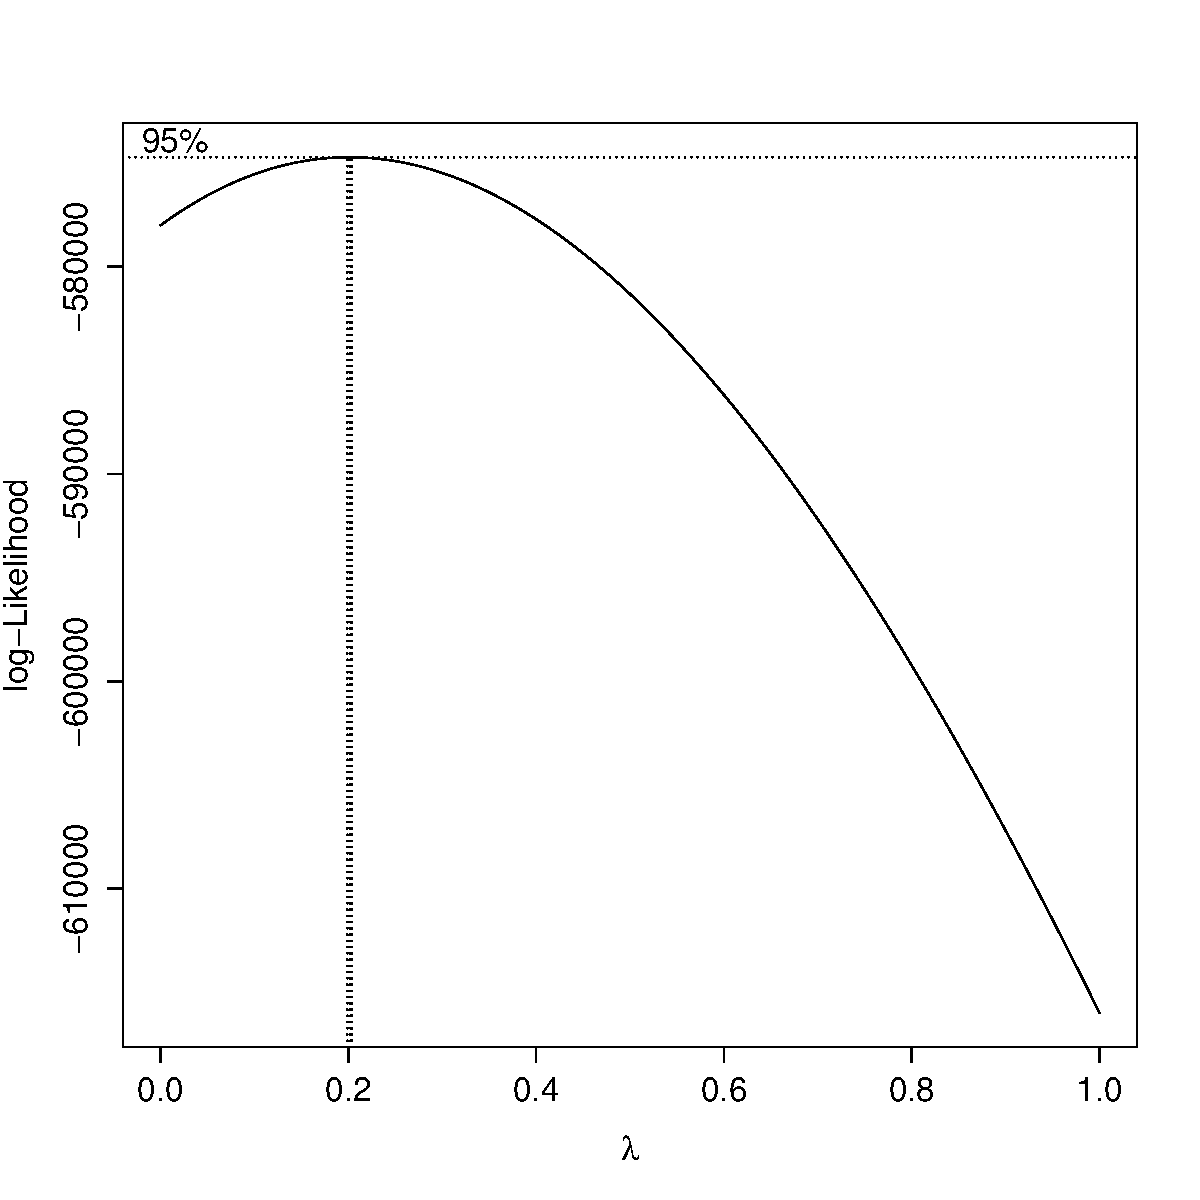
\includegraphics[width=0.4\linewidth]{figs/LogLikelihood-Backers.pdf}
	}
	\hspace{1cm}
	\subfigure[Value of $\lambda$ in regression model for predicting amount of funding] % caption for subfigure b
	{
		\label{fig:lambdaFunding}
		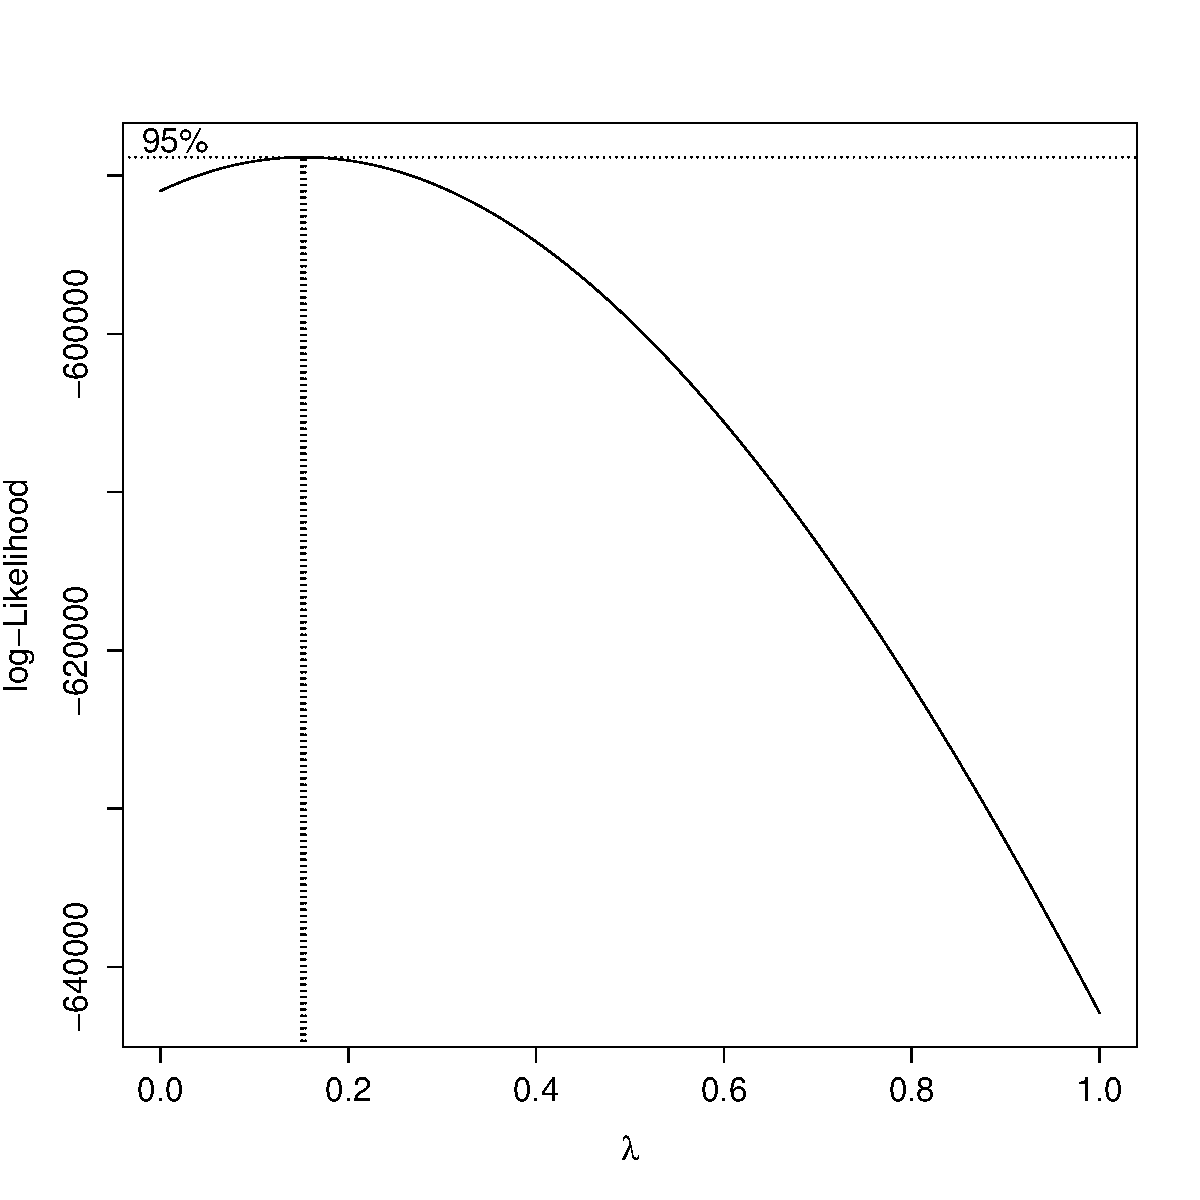
\includegraphics[width=0.4\linewidth]{figs/LogLikelihood-Funding.pdf}
	}
	\caption{Value of $\lambda$ in 2 models: predicting number of backers and the amount of funding}
	\label{fig:LambdaFig}
	\vspace{-10pt}
\end{figure*}

Figure \ref{fig:LambdaFig} shows the change of loglikelihood when varying the $\lambda$ value. For building the model to predict number of backers, we observed in Figure \ref{fig:lambdaBackers} that at $\lambda-0.2$, the loglikelihood function achieve the highest value. With regard to the model of predicting the amount of funding, it is shown in Figure \ref{fig:lambdaFunding} that we obtained the maximum value of loglikelihood when $\lambda = 0.18$. Hence, we set $\lambda = 0.2$ and 0.18 in the models of predicting number of backers and the amount of funding, respectively.

As a result, we fit the following model for predicting number of backers:
\begin{equation}
\label{equa:model1 }
\begin{aligned}
	Y_{backers}^{0.2} = \beta_0 + \beta^TX + \epsilon 
\end{aligned}
\end{equation}

And the model for predicting the amount of funding need to be fitted is as following:
\begin{equation}
\label{equa:model2}
\begin{aligned}
	Y_{funding}^{0.18} = \beta_0 + \beta^TX + \epsilon
\end{aligned}
\end{equation}
where $\epsilon$ is the random error and $\epsilon\sim N(0, \sigma^2)$ 

\textbf{Predicting how many backers will back for a Kickstarter project:} we fit our proposed model given in Equation (\ref{equa:model1 }). Then we compare the result with linear regression model and extreme gradient boosting for linear model. Figure \ref{fig:BackerRegressionResult} shows RMSE of 3 models for predicting how many backers will back for a Kickstarter project. We note that linear regression model obtained lowest result with RSME of 66.9. Boosting linear regression with Xgboost gained higher result with RSME of 28.7. However, comparing to these two models, our approach obtained the best result with lowest RSMSE of 23.7.

%\begin{figure}%[!ht]	
%	\centering
%	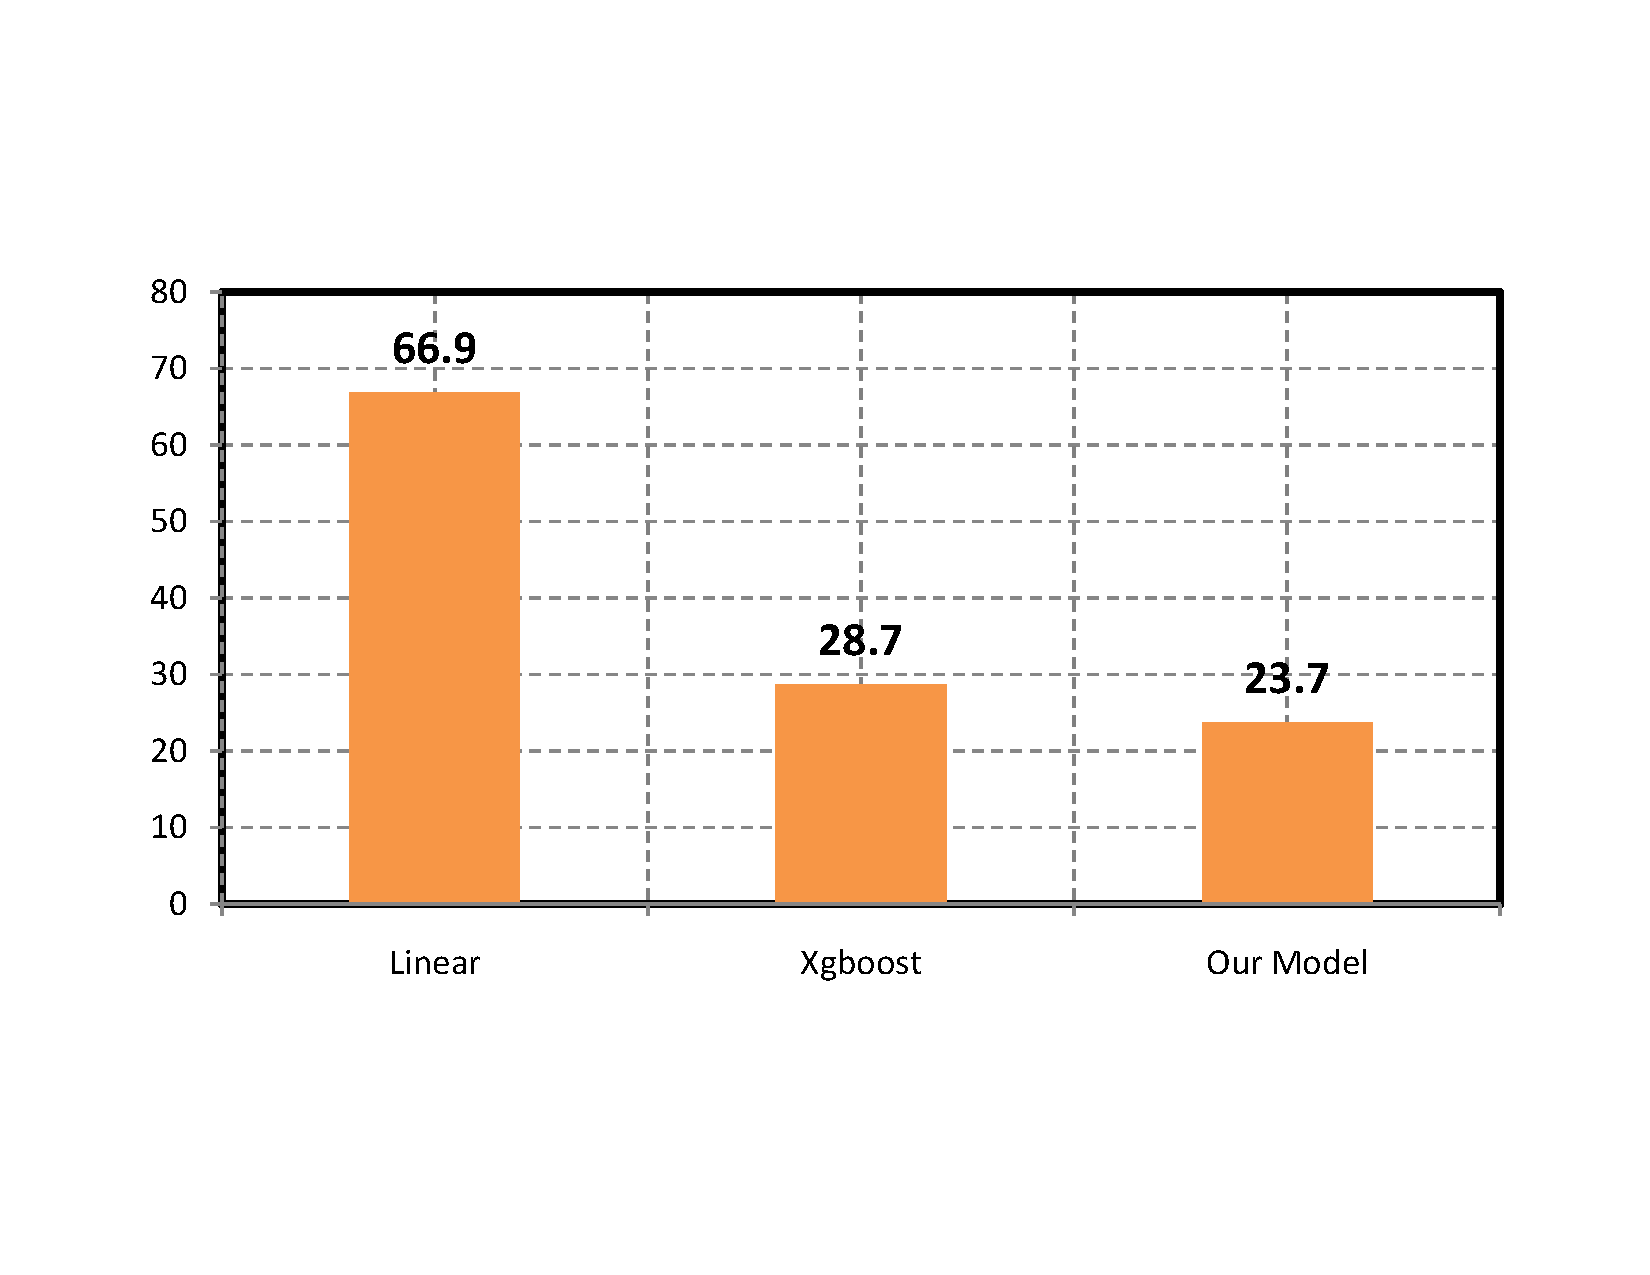
\includegraphics[width=\linewidth]{figs/BackerRegressionResult.pdf}
%	\caption{RMSE of different models for predicting how many backers will back for a Kickstarter project}
%	\label{fig:BackerRegressionResult}
%	\vspace{-10pt}
%\end{figure}

\begin{figure*}[!ht]
	\centering
	\subfigure[Predicting how many backers will back for a Kickstarter project] % caption for subfigure a
	{
		\label{fig:BackerRegressionResult}
		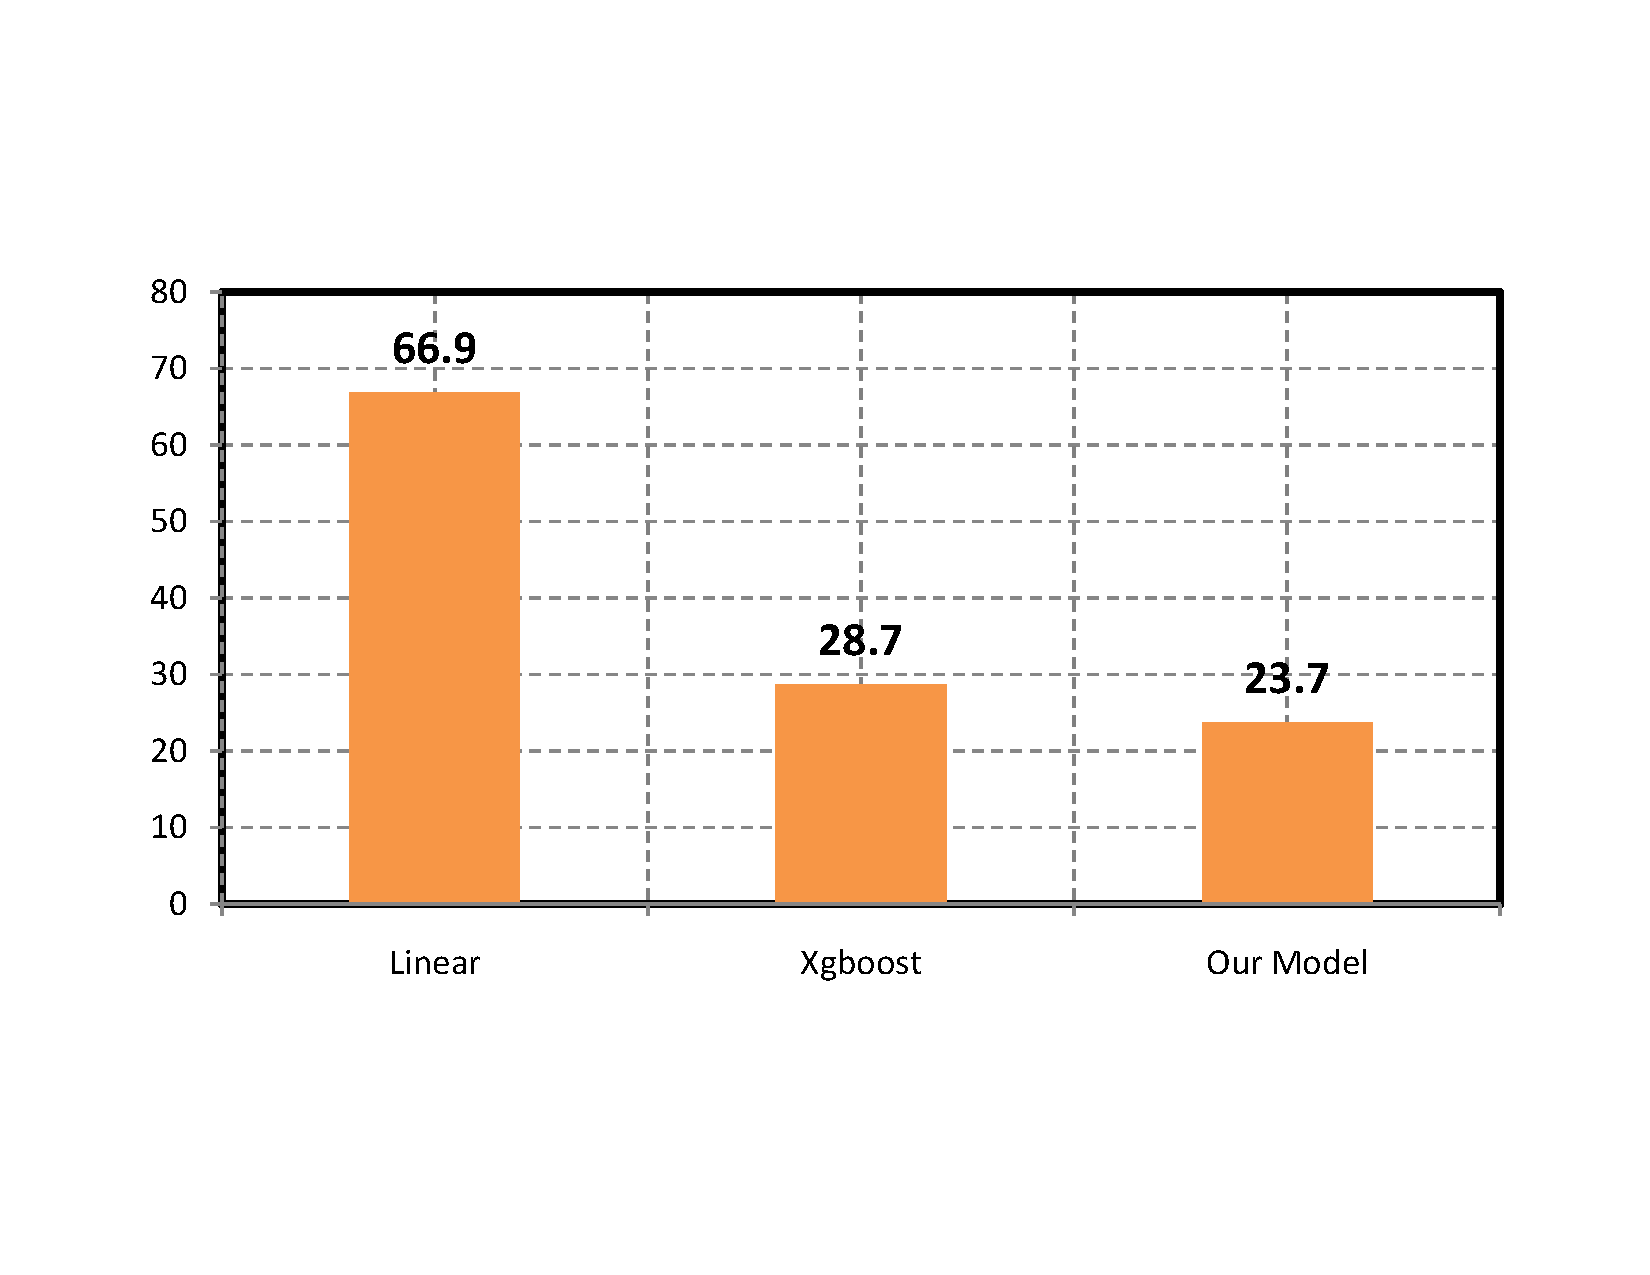
\includegraphics[width=0.4\linewidth]{figs/BackerRegressionResult.pdf}
	}
	\hspace{1cm}
	\subfigure[predicting how much funding a Kickstarter project can receive] % caption for subfigure b
	{
		\label{fig:FundingRegressionResult}
		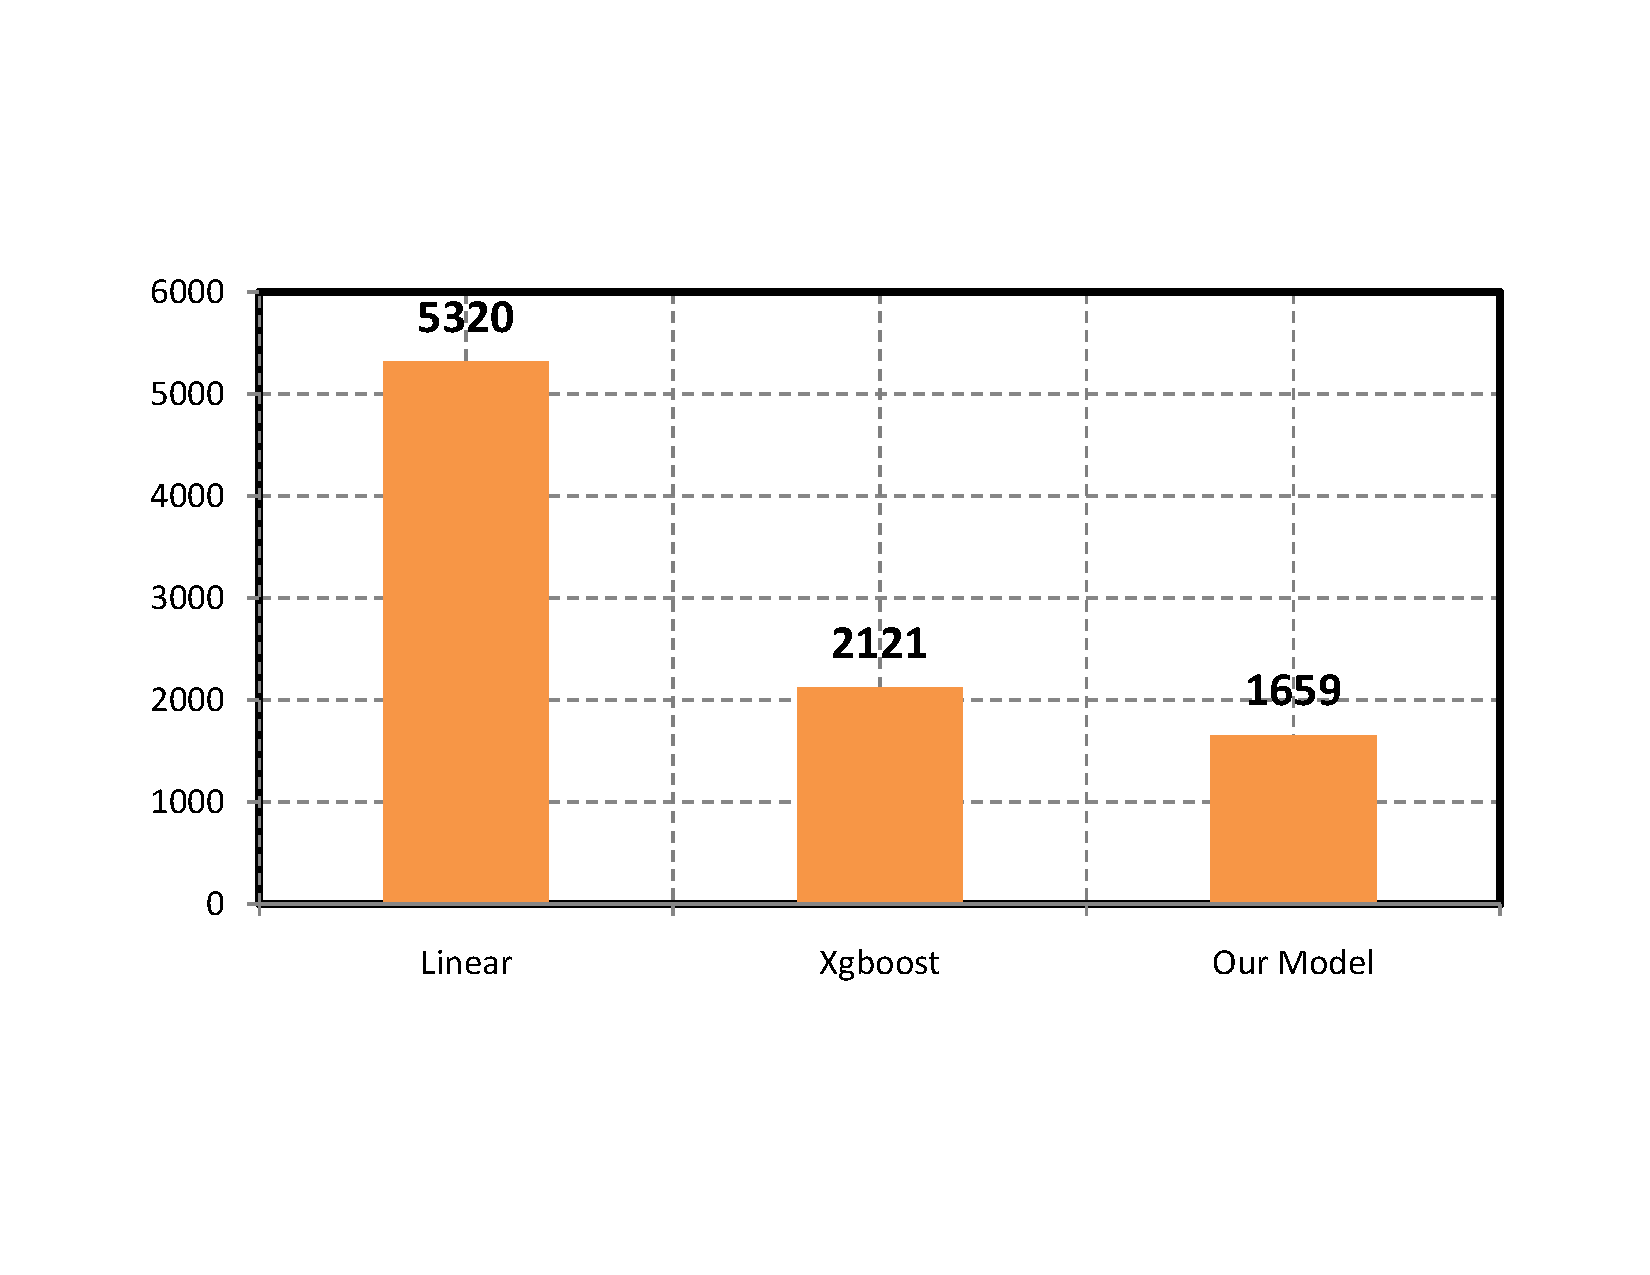
\includegraphics[width=0.4\linewidth]{figs/FundingRegressionResult.pdf}
	}
	\caption{RMSE of different models for (a) predicting how many backers will back for a Kickstarter project, and (b) predicting how much funding will a Kickstarter project receive}
	\label{fig:RegressionResult}
	\vspace{-10pt}
\end{figure*}

\textbf{Predicting the amount of funding a Kickstarter project can receive:} we fit our proposed model given in Equation (\ref{equa:model2}) to predict how much funding a Kickstarter project can be funded. We also compared our result with the results we got from linear boosting of Xgboost and linear regression. Figure \ref{fig:FundingRegressionResult} shows RMSE result of 3 models. We notice that our model outperformed linear regression and Xgboost for linear model with lowest RMSE of 1,659. This value is the average error of predicting the amount of funding for a Kickstarter project. 

%\begin{figure}%[!ht]
%	\centering
%	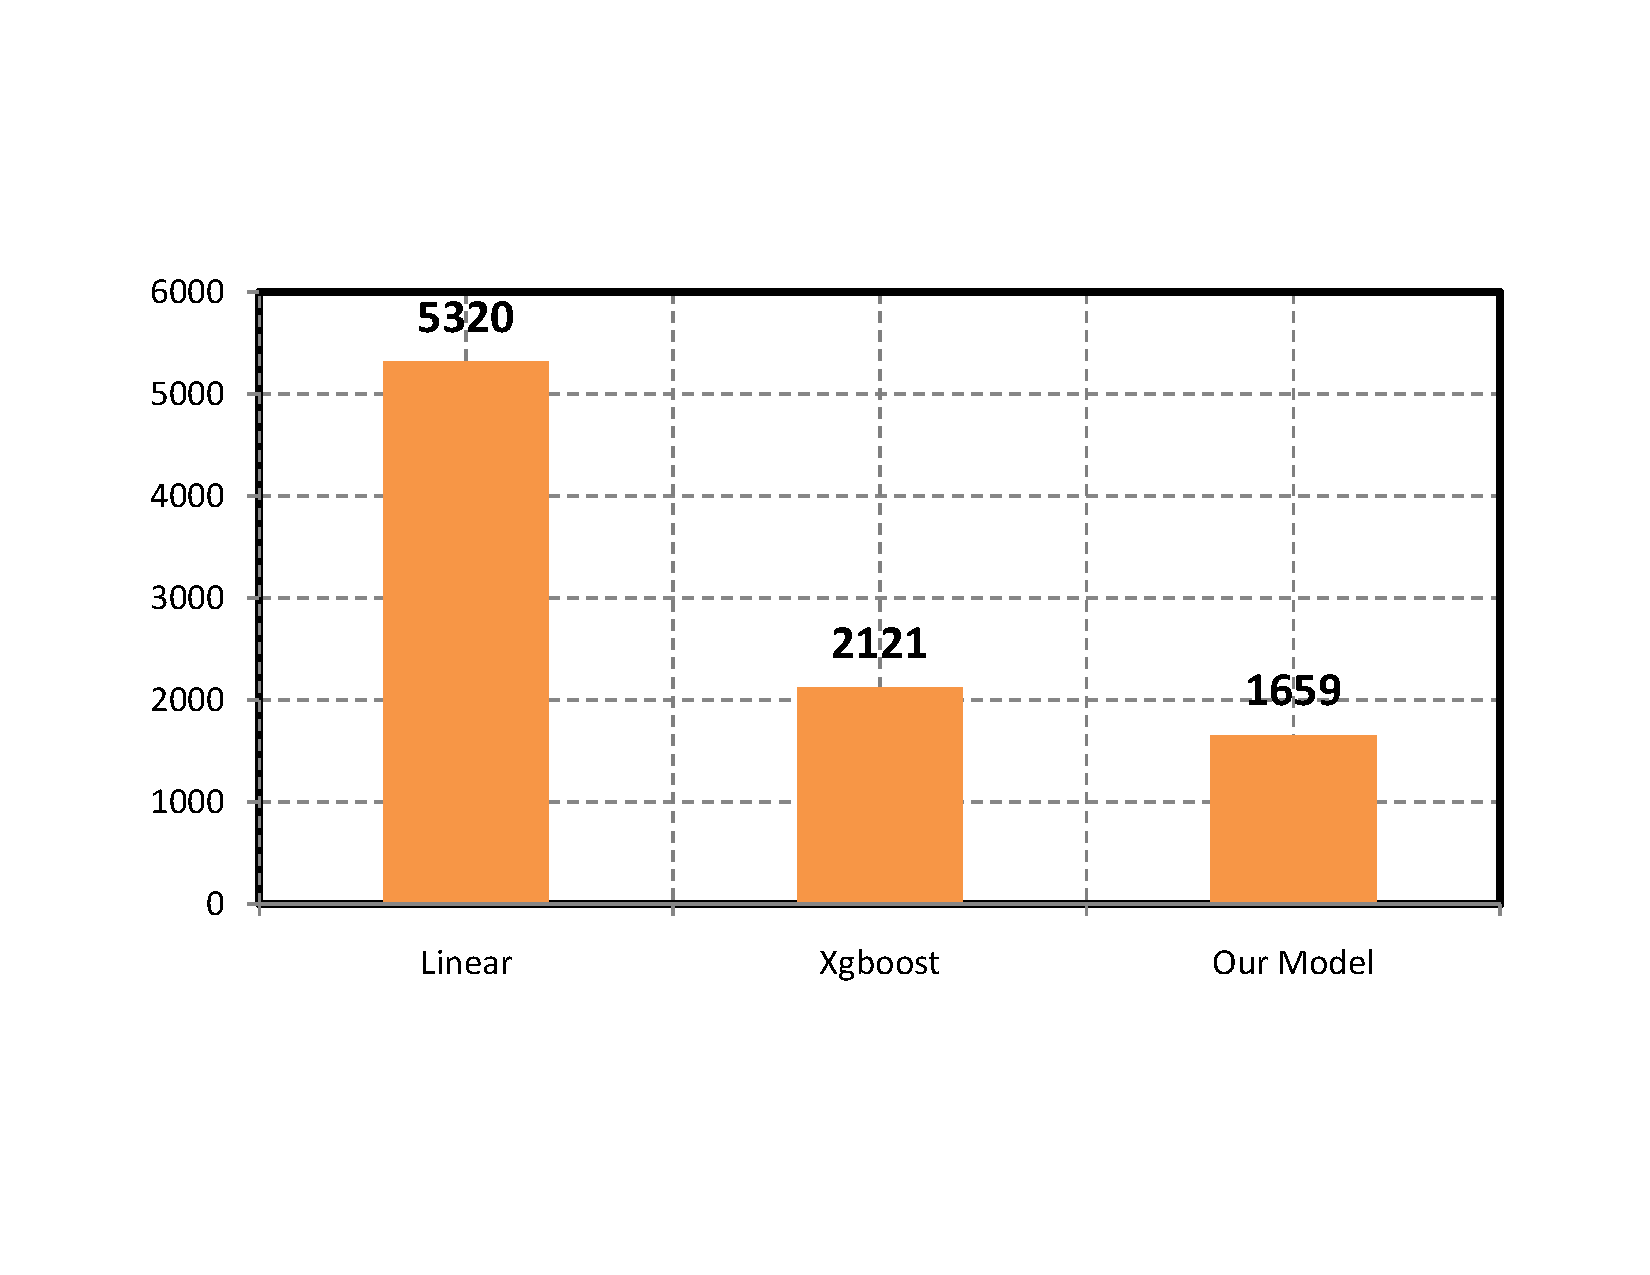
\includegraphics[width=\linewidth]{figs/FundingRegressionResult.pdf}
%	\caption{RMSE of different models for predicting how much funding will a Kickstarter project receive}
%	\label{fig:FundingRegressionResult}
%	\vspace{-10pt}
%\end{figure}
\section{Conclusion}
\section{Future Works}

%
% The code below should be generated by the tool at
% http://dl.acm.org/ccs.cfm
% Please copy and paste the code instead of the example below. 
%

%
% End generated code
%

%
%  Use this command to print the description
%
\printccsdesc

% We no longer use \terms command
%\terms{Theory}

\keywords{Kickstarter; crowdfunding}


\bibliographystyle{abbrv}
\bibliography{sigproc}

\end{document}
